\chapter{Results and Discussion} \label{Result}
 With the suitable algorithms implemented, in this section the parameters of the algorithms are further discussed. As the data of the virtual sensors are dependent on its preferences in the Unity3d scene, they are documented in subsection \ref{Parameters}. Subsequently the performance of the system is evaluated by taking the latency of every processing step. The tests are strongly focused on the median latency and reliability in terms of timing inaccuracies and scattering of the data generation, transmission and processing. The tests that are conducted in the following can be divided into the test of the modules which goes along with the integration of the modules in subsection \ref{latency}, the test to proof the successful integration of parts in subsection \ref{intpart} and the validation of the software as a whole in subsection \ref{validate}.
 
 \section{Sensor Parameters} \label{Parameters}
 The virtual sensors as implemented in the Unity3d scene have to generate data about its digital environment by reproducing the physical properties of real sensors. Inherent to this approach is the limitations that are set by the processing power of the unit that calculates the virtual sensors data. Therefore, in addition to the values that can be derived from real sensors, the performance of the system has to be observed when for example increasing the resolution of a sensor to resemble an analogous sensor signal by means of discrete digital values. The settings of the sensors and data processing algorithms values are determined experimentally and merely provide an example for the possibilities of the overall system architecture. Therefore in the following the validation of the values is conducted on a qualitatively basis without comparing the performance effects of different sensor settings. \\
 
 The resolution of the virtual \ac{RADAR} is an example for the necessity to deviate from the real sensor as proposed before. To realize an object detection in a range of several kilometres with a detection rate that equals that of an analogous \ac{RADAR}, the digital \ac{RADAR}'s angular resolution exceeds the processing power of a common computer. Thus its detection range is limited to about 100m for objects below four meters in the current implementation. Table \ref{tab_radarsens} provides an overview of the settings of the \ac{RADAR}. One beam of the \ac{RADAR} is five degrees wide in azimuth and 15$\degree$ wide in altitude. The resolution of one beam is 30x2 raycasts. For the detection of objects close to the \ac{RADAR}'s origin the resolution proved to be sufficiently detailed. However, after exceeding a certain range, small objects are able to pass the \ac{RADAR}'s rays undetected due to the increasing space between subsequent rays. To increase the detection rate of objects, providing them with a very high reflection value of about 100 provided good results when applying the \ac{SOCA-CFAR} filter.\\ 
 
 The settings of the filter that proved to be most effective are documented in table \ref{tab_filter}. A total of 100 cells are taken into consideration to compute the decision whether the \ac{CUT} is classified as an target object or not. Ten cells that are five to the right and five to the left of the \ac{CUT} are ignored and thus decrease the chance that signals of objects are taken into consideration when computing the noise average. The false detection rate is set to 0.1. In contrast to a fixed threshold, the \ac{SOCA-CFAR} provides usable results even when changing the settings of the virtual \ac{RADAR} which for example results in an increased overall reflection value. That can be considered as an effect of the dynamic threshold    calculation.                                                                                                                                                                                                                                                                                  
  
  \begin{figure}[!htb]
 	\begin{minipage}[t]{0.48\textwidth}	
 		\begin{table}[H]	
 			\centering
 			\caption{\ac{RADAR} sensor values}
 			\begin{tabular}{l l } 
 				\midrule\midrule
 				Unity3d  & Value\\ 
 				\midrule
 				Cell Azimuth Extension  &5.0\\
 				Cell Extension & 4  \\
 				Cell Altitude Extension & 15\\
 				Burst Vertical Resolution & 30\\
 				Burst Horizontal Resolution & 2
 			\end{tabular}
 			\label{tab_radarsens}
 		\end{table}
 	\end{minipage}\hfill
 	\begin{minipage}[t]{0.48\textwidth}
 		\begin{table}[H]
 			\centering
 			\caption{Filtering values}
 			\begin{tabular}{l l } 
 				\midrule\midrule 
 				SOCA-CFAR  & Value\\ 
 				\midrule
 				Training Cells&100 \\	
 				Guard Cells&10 \\
 				False Detection Rate& 0.1
 			\end{tabular}
 			\label{tab_filter}
 		\end{table}
 	\end{minipage}
 \end{figure}
 The physical principle of operation of the \ac{LIDAR} allows virtual data generation without further transformation and approximation. Thus, the data generation in the simulation can forgo without substantial compromises. As listed in table \ref{tab_lidarsens} the \ac{LIDAR} is set to about 345000 points with a frequency of two Hertz. The horizontal and vertical resolution are 0.25$\degree$ per ray with an field of view of 360$\degree$ and 60$\degree$ respectively. The procession of the points with the \ac{DBSCAN} algorithm yields the most promising results with the settings in table \ref{tab_cluster}. The values have been determined experimentally with adjustments taken in comparison with the objects spatial limitations as visible in the Unity3d scene. An $Eps$ value of one equals to points being considered as neighbours with an distance of below one meter to each other. $MinPts$ set to ten indicates that a minimum of ten points is required in a cluster to be considered as such. The resolution of the bounding box is a further value that can be set. With applications prioritising accuracy, the resolution can be set higher and thus allow for boxes that frame the data more precisely. However, in situations that require a highly responsive system, compromising the accuracy by decreasing the resolution to higher bounding box values can lead to a higher performance in terms of processing time. The value of three that equals to three meters provides a sufficient accuracy without using to much processing time.
 \begin{figure}[!htb]
 	\begin{minipage}[t]{0.48\textwidth}	
 		 \begin{table}[H]	
 			\centering
 			\caption{\ac{LIDAR} sensor values}
 				\begin{tabular}{l l } 
 				\midrule\midrule
 				Unity3d  & Value\\ 
 				\midrule
 				Horizontal Resolution	& 0.25\\
 				Vertical Resolution& 0.25 \\
 				Vertical Field of View	& 60\degree
 				\end{tabular}
 			\label{tab_lidarsens}
 		\end{table}
 	\end{minipage}\hfill
 	\begin{minipage}[t]{0.48\textwidth}
 		 \begin{table}[H]
 			\centering
 			\caption{Clustering values}
 				\begin{tabular}{l l } 
	 			\midrule\midrule 
 				DBSCAN  & Value\\ 
 				\midrule
 				Eps&1 \\	
 			    MinPts&10 \\\\
 			    
 				\midrule\midrule
 				Bounding Box & Value\\
 				\midrule
 				Resolution & 3
 				\end{tabular}
 			\label{tab_cluster}
 		\end{table}
 	\end{minipage}
 \end{figure}
 By choosing the resolution and compression of the rendered image from the Unity3d scene, the data size of the visual environment information can be reduced or increased. As shown in table \ref{tab_imagesens}, 640 pixel in width and 480 pixel in height are chosen as values for the image resolution together with a jpeg compression. These values provide enough details for the subsequent line extraction and at the same time allow for an acceptable procession time. For the edge detection and line extraction, table \ref{tab_extraction} provides information of the used variables. The algorithm for the edge detection as proposed by Canny uses 170 for a first threshold and 260 as a second threshold. With an value above one for $Rho$ as the distance in pixels between sampled pixels and a $Theta$ of one as the angular distance in which lines through edge points are computed, the Hough algorithm provides a sufficient computation time. To decrease the false alarm rate, the $Threshold$ is set to 190. Increasing this value results in a higher amount of lines with the same value in the Hough feature space for an edge to be considered a line in the Hough image space.
 \begin{figure}[!htb]
	\begin{minipage}[t]{0.48\textwidth}	
		\begin{table}[H]	
			\centering
			\caption{Image sensor values}
			\begin{tabular}{l l } 
				\midrule\midrule
				Unity3d  & Value\\ 
				\midrule
				Width & 640 \\
				Height & 480 \\
				Compression & Jpeg\\
				
			\end{tabular}
			\label{tab_imagesens}
		\end{table}
	\end{minipage}\hfill
	\begin{minipage}[t]{0.48\textwidth}
		\begin{table}[H]
			\centering
			\caption{Line extraction values}
			\begin{tabular}{l l } 
				\midrule\midrule 
				Canny  & Value\\ 
				\midrule
				Threshold 1 &170 \\	
				Threshold 2 & 260 \\
				\midrule\midrule 
				Hough  & Value\\ 
				\midrule
				Rho & 1.1 \\	
				Theta & 1\degree\\
				Threshold & 190
			\end{tabular}
			\label{tab_extraction}
		\end{table}
	\end{minipage}
\end{figure}



	\section{Module and Module Integration Test}\label{latency}
	The specifications of the hardware that is used to test the system is given in table \ref{tab_hardware}. With 30 GiB of random access memory, 16 cores at 3.60 GHz and a RTX series graphics card, the system can be considered as being up to date. As an operating system Ubuntu LTS is used. This Linux derivative has the advantage that it is supported by \ac{ROS2} as well as Unity3d.	
	
	\begin{table}[H]
		\centering	
		\caption{Hardware used for testing}
		\begin{tabular}{l l } 
			\toprule
			Category  & Type\\ 
			\midrule
			Processor & 			Intel Core i9-9900KF CPU @ 3.60GHz x 16 \\ 
			Random Access Memory & 	30GiB\\
			Graphics Card & 		Nvidia TU104 GeForce RTX 2070 SUPER\\
			Operating System & 		20.04.2 LTS Ubuntu\\
			\bottomrule	
		\end{tabular}
		\label{tab_hardware}
	\end{table}

	To test the modules that are represented by methods in Unity3d and ROS2, the time each method takes to be executed is saved multiple times. As the system modules are dependent on each other, the test is executed with a function-able system without executing single methods in an isolated environment. Therefore, module and integration test are conducted simultaneously. Table \ref{tab_abb} in appendix \ref{Attachtable} depicts the single methods and average times of execution of these methods. As a benchmark for the execution time in the Unity3d system, the default physics engine update time of 20ms is used. Values below 20ms allow an event calculation as intended by the engine and enable Unity3d to render a consistence visual simulation representation. The benchmark of the \ac{ROS2} process time is the frequency of the sensors data generation e.g. the \ac{LIDAR} sensor is set to 2 Hertz.\\
	
    The processor and \ac{GPU} utilization in the system during the tests is shown in table \ref{tab_cpuload}. For the CPU, the load in three system states is taken with the tool \textit{htop}. With a total of 16 cores, a value of 16 results in the CPU being full loaded. Values above 16 result in queued processes. The system in idle mode uses 60\% of one core and the system with an active Unity3d simulation and running ROS2 nodes uses six cores and 56 \% of the seventh core. Regarding the GPU load that is measured with \textit{nvidia-smi}, only 49\% is used with Unity3d and ROS2 running. It can be stated, that the CPU and GPU processing power constitute no limitation for conducting tests on the system.
		
		\begin{table}[H]
		\centering	
		\caption{CPU and GPU load}
		\begin{tabular}{l l } 
		\midrule\midrule 
		System processes & CPU Load (max 16) $\varnothing1min$\\ 
		\midrule
		Idle			 & 0.6 \\	
		Unity3d 		 & 3.91 \\
		Unity3d and ROS2 & 6.56 \\
		\midrule\midrule
		System processes & GPU Load (max 100\%)\\
		\midrule
		Unity3d and ROS2 & 49\% \\
	\end{tabular}
		\label{tab_cpuload}
	\end{table}

	To test the implementation of the modules in the system, the average execution time of the methods for the \ac{IMU}, Image, \ac{RADAR} and \ac{LIDAR} in Unity3d and \ac{ROS2} is taken. Figure \ref{fig_time} depicts these values. In the first category with execution times from (a) to (d), the methods for the \ac{IMU} data (a) equals to zero as the average is below the vertical axis that is logarithmic scaled in milliseconds. (a), (b) and (c) are below the 20ms with which Unity3d updates its physics per default. The calculation of the \ac{LIDAR} data (d) exceeds 20ms with a value of 69ms. This makes a more detailed analysis  necessary to narrow down on the methods that are responsible for the high computation time.\\
	
	The second category in figure \ref{fig_time} is represented by the \ac{ROS2} subsystem. The according values for (e) to (h) represent the time that is required to process and visualize the data of the sensors. With a value of above 72ms, the \ac{IMU} (e) with an update rate of 50 Hertz exceeds its benchmark value of 20ms values by 52ms. The same counts for the calculation of the \ac{LIDAR} data (h). With an update rate of 500ms, the processing time surpasses the defined benchmark by 517ms. Both the methods of (e) and (h) are looked upon in greater detail in the following. (f) and (g) can be considered as performing well in comparison to its update rate of 500ms. 
	\begin{figure}
		\begin{centering}
			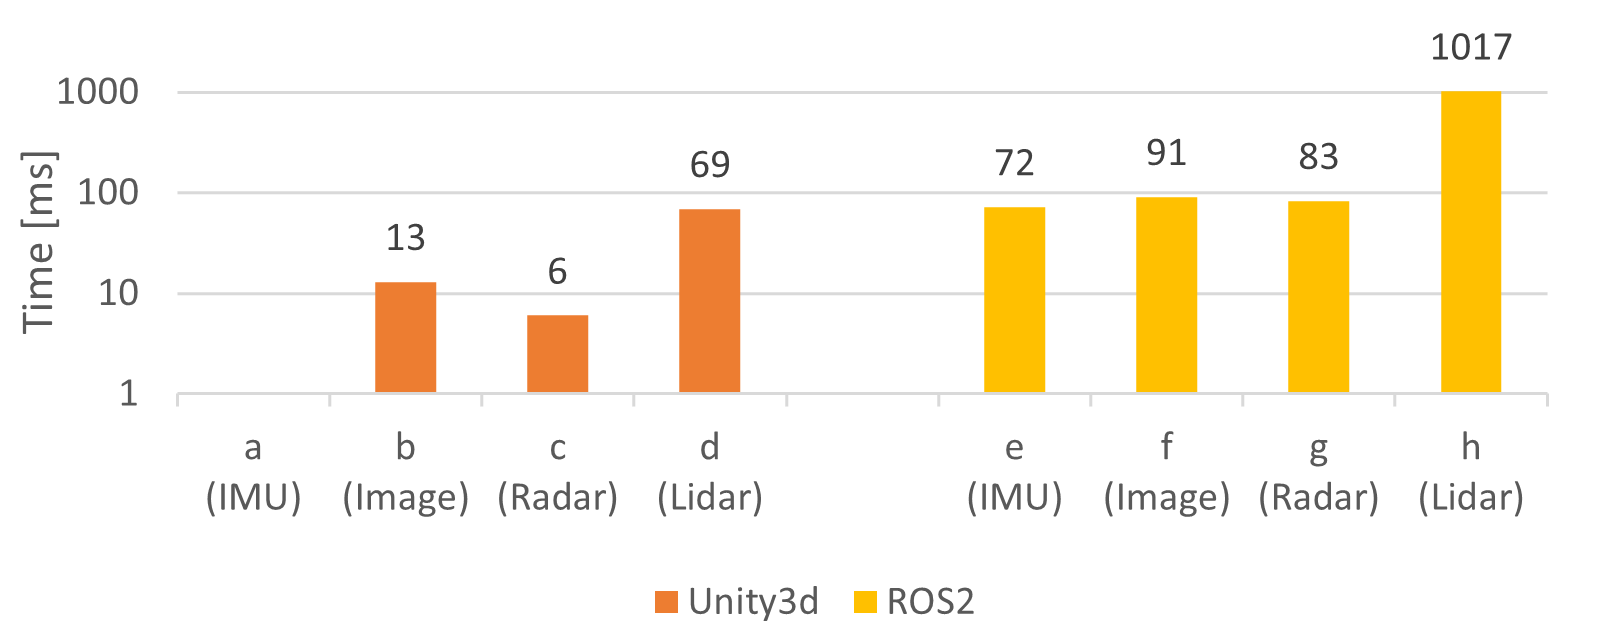
\includegraphics[width=0.75\textwidth]{Bilder/Time.PNG}
			\caption{Methods average execution time (total of 165000 execution)}
			\label{fig_time}%Label für das Referenzieren 
		\end{centering}
	\end{figure}
	
	Figure \ref{fig_Unity3d1} provides more detailed information about the execution time of methods in Unity3d with a box and whisker plot. The figure is divided into two plots with the plot to the left describing the methods execution time in milliseconds up to 18 milliseconds and the plot to the right methods with a longer execution time up to 180 milliseconds. A total of fourteen methods of the categories Radar, Image, \ac{IMU} and Lidar are investigated over a total of 126000 executions with an update frequency of two Hertz with the \ac{IMU} being an exception with 50 Hertz. In the plot to the left, the raycast of the \ac{RADAR} (1b) takes the longest time by comparison of medians. However, with 4 milliseconds this value can be considered as sufficient low compared to the time of 20ms with which the the physics engine of Unity3d calculates new data per default. In terms of reliability, there are outliers which are higher than the 4ms of (1b). This is of importantance in particular as they compromise the reliability of data generation in a fixed time. Especially publishing the \ac{IMU} data (1i) stands out in terms of difference from the median to the outliers. The longest execution time of (1i) is around 17ms. However, when using the benchmark of the repetition rate of the physics update, this value can be considered as sufficiently fast to avoid missing physics events.\\
	
	The plot to the left depicts the three most time consuming methods on Unity3d with the data generation of the \ac{LIDAR} (2a), publishing the data of the \ac{LIDAR} (2b) and generation i.e. rendering of the image. By exceeding the physics update repetition rate, methods (2a) and (2c) show a very limited range of the times of the outliers. In contrast executing (2c) can take up to 170ms with a median of 13ms. It can be assumed that for the three outliers that are considerably higher than the median an exception occurs e.g. other processes are scheduled to be executed on the same processor core as (2c). To summarize, for a higher performance in Unity3d, (2b) has to be optimized towards a higher overall performance and modifications in the system should lead to avoidance of the peak values of (2c).\\
	
	%However, as the update frequency of (2a),(2b) and (2c) is two Hertz, the implementation as tested is sufficient for the application with the backdraw of missing some physic events and visual representations. This effect should be minded for appliances that require a simulation  \\ 
	
	\begin{figure}
		\begin{center}
			\resizebox{.9\textwidth}{!}{%
				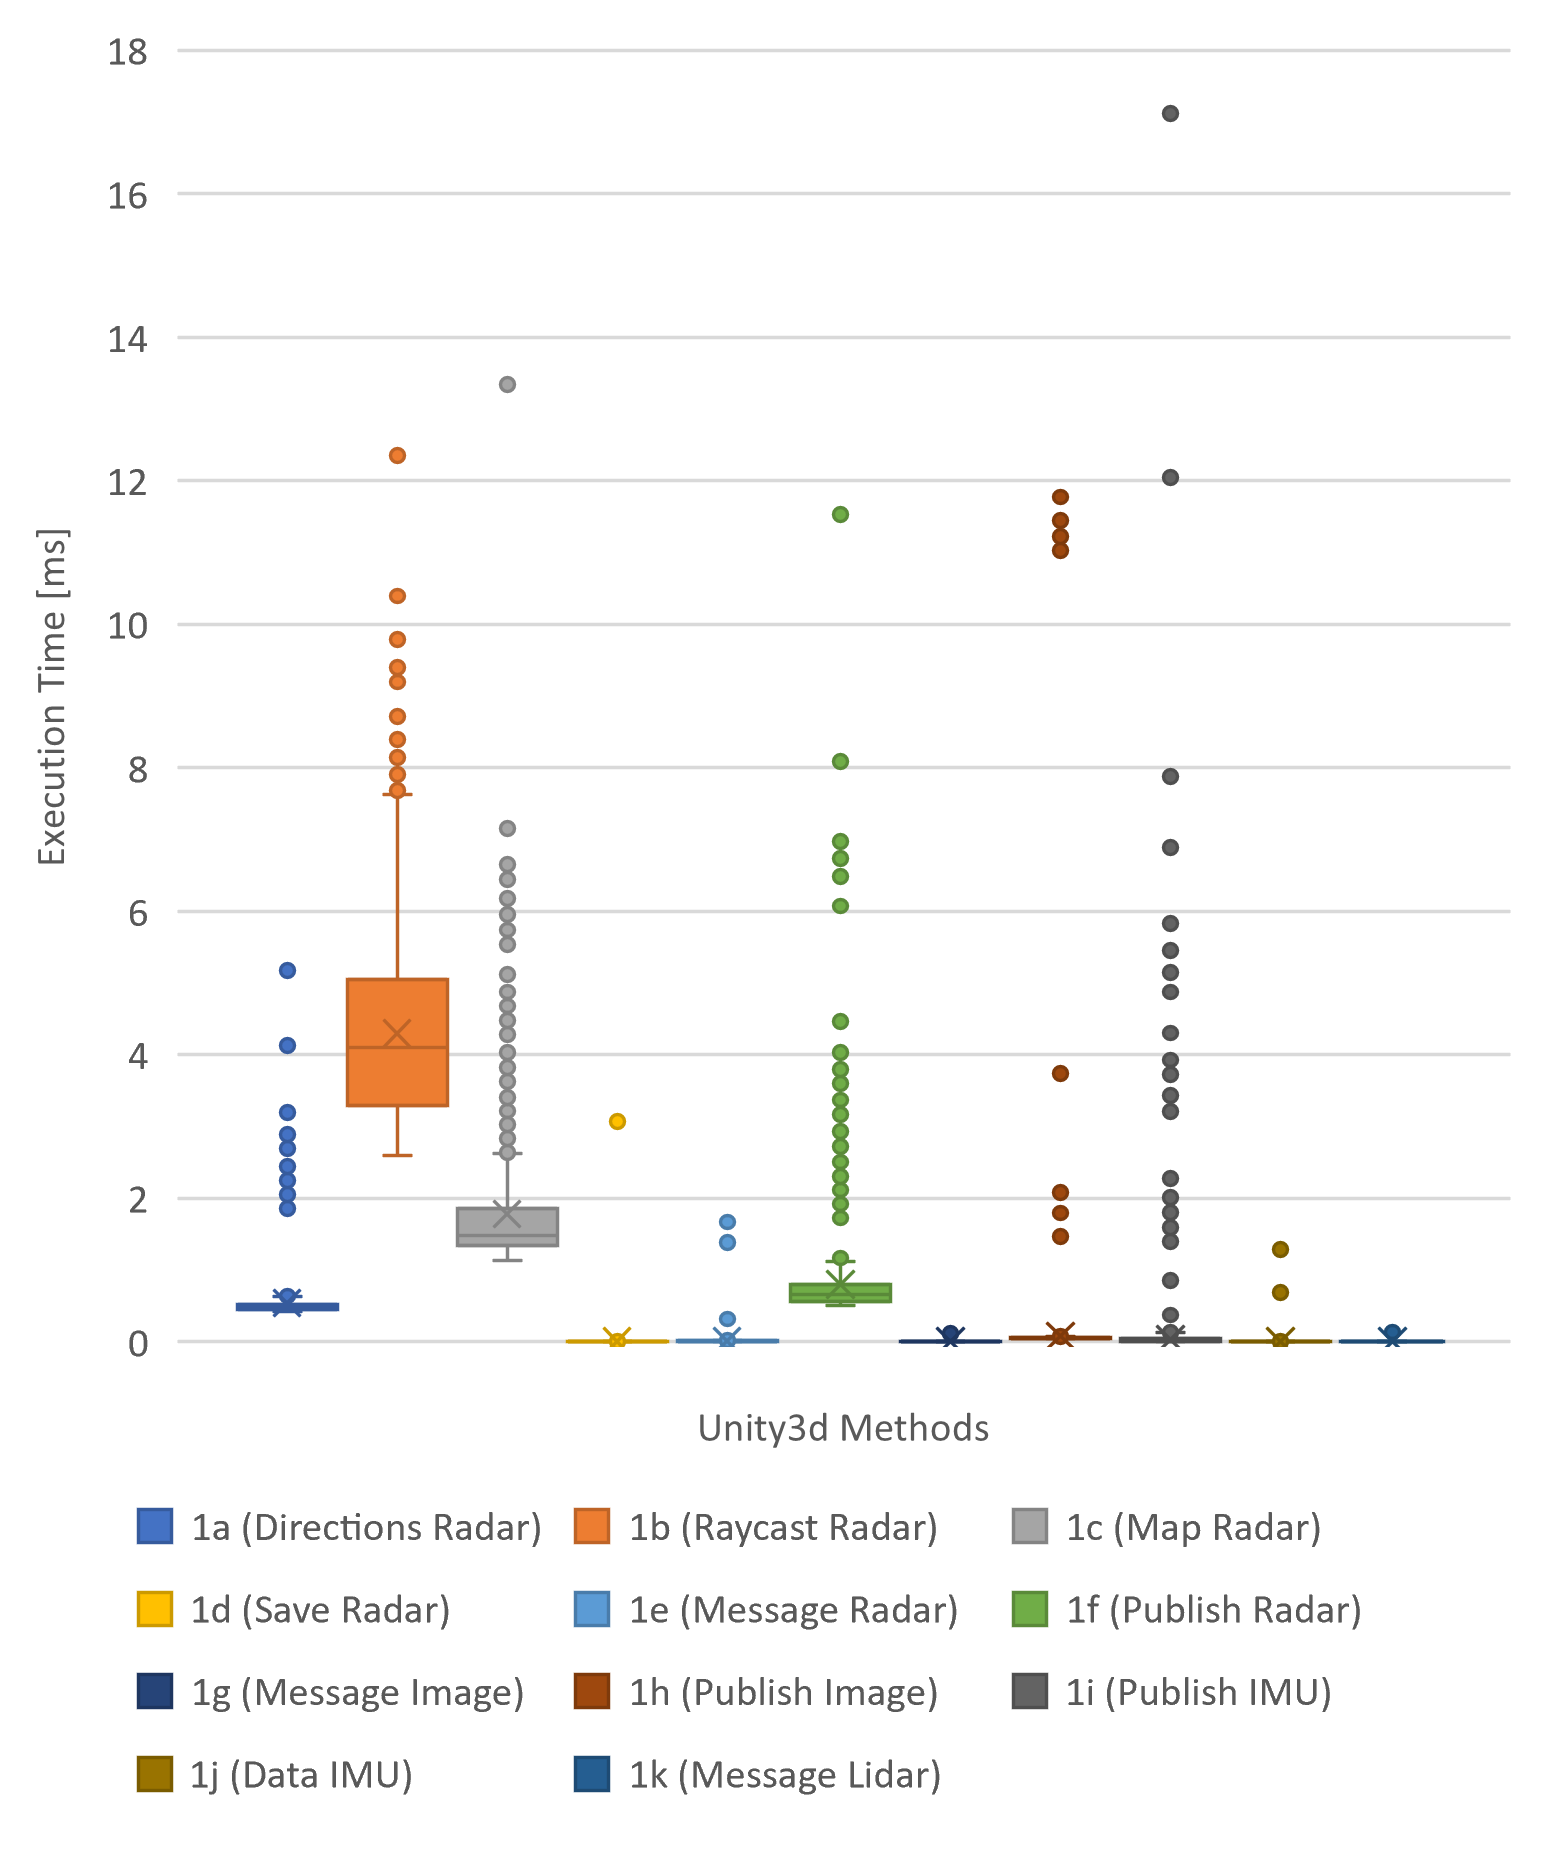
\includegraphics[height=3cm]{Bilder/Unity3d1.png}%
				\enskip
				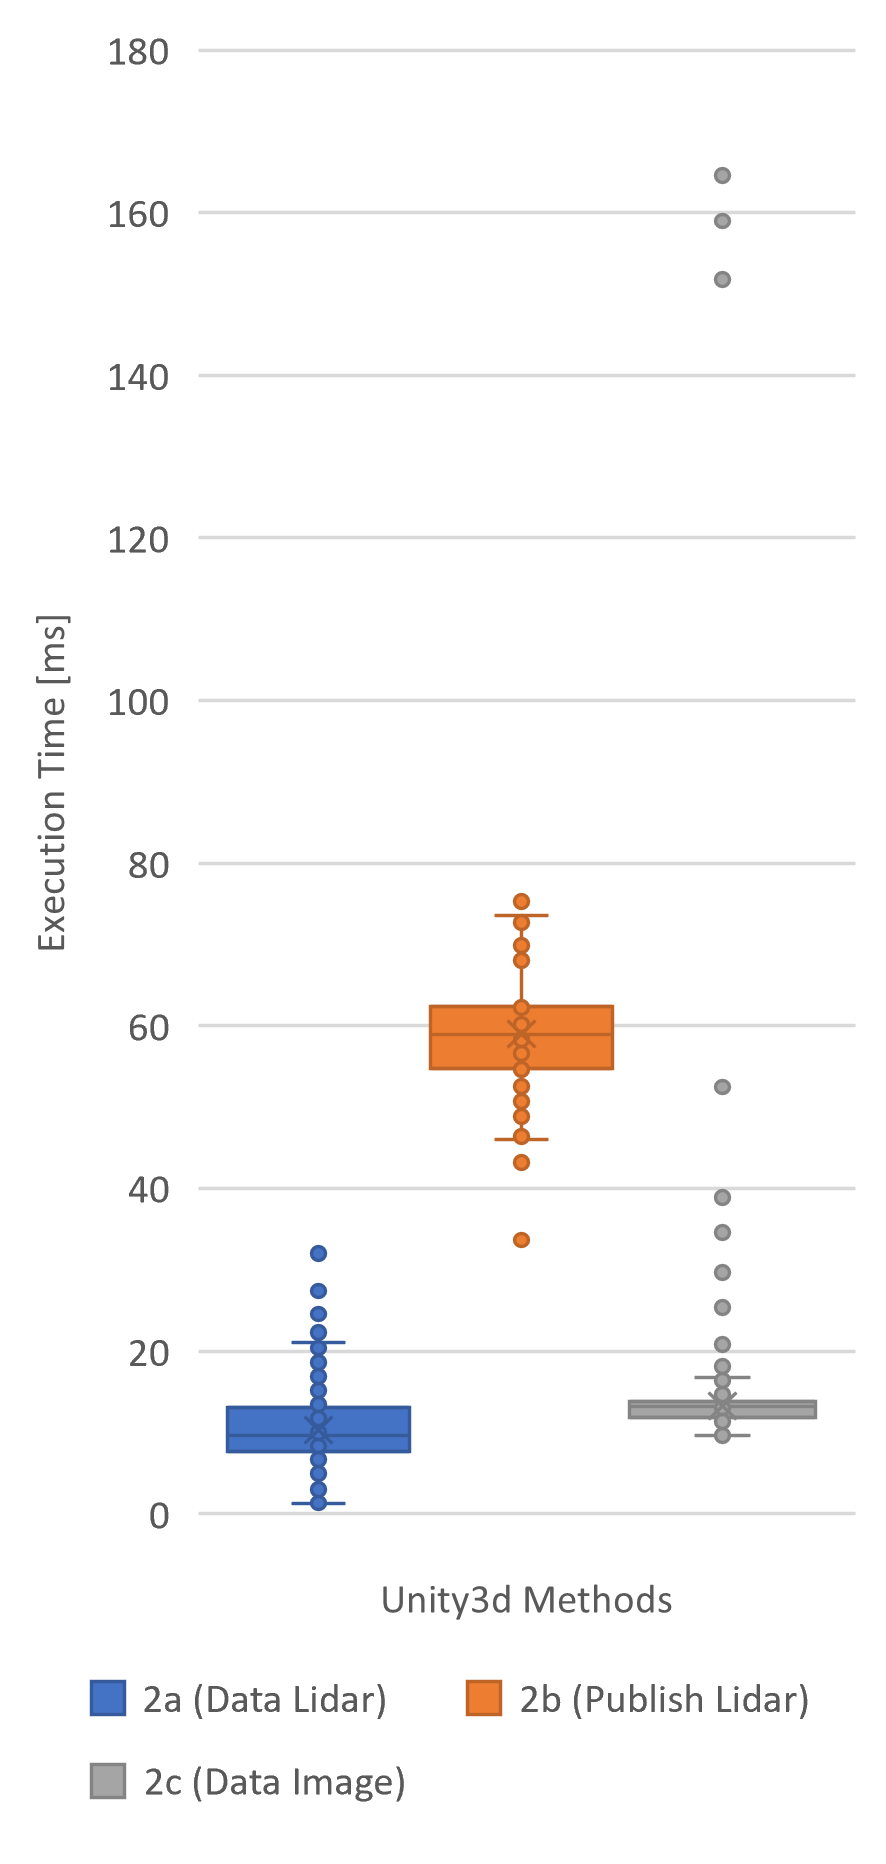
\includegraphics[height=3cm]{Bilder/Unity3d2.png}%
			}
			\caption{Unity3d methods time (total of 126000 executions)}
			\label{fig_Unity3d1}%Label für das Referenzieren 
		\end{center}
	\end{figure}
  
   For the methods that are executed in \ac{ROS2} figure \ref{fig_Ros21} provides two figures with a similar structure to figure \ref{fig_Unity3d1}. The figure to the left plots data up to 300ms and the plot to the right data up to 3s in a box and whisker representation of about 27300 executions. Again the methods that are depicted can be looked up in appendix \ref{Attachtable} in table \ref{tab_abb}. In figure \ref{fig_Ros21}, (3a) to (3h) process times at below 300ms even for exceptional outliers are shown, which is sufficient for the application at hand. Going into further detail, method (3g) that computes the bounding boxes for the \ac{LIDAR} data is noteworthy as it shows an comparable high median of just below 200ms. Thus (3g) provides a first method that can be optimized towards a lower computing time to minimize the \ac{LIDAR} data processing time.\\ 
   
    In the plot to the right it becomes clear that the execution times of (4a) to (4b) can exceed 500ms. That is a critical limit as the frequency from the data generation in Unity3d is set to two Hertz. With the methods execution time above 500ms the \ac{ROS2} network is not able to process the data in time which can lead to data being ignored. Upon further investigation, it becomes clear that these methods solely visualize data. As the data visualization is implemented with the matplotlib library for Python, finding another library more suited to plot data in a repeated cycle provides a way to improve the time needed for visualization. A further chance of improvement is given by the visualization of already processed data e.g. visualizing the bounding boxes of the \ac{LIDAR} data instead of the whole point cloud.
	\begin{figure}
		\begin{center}
			\resizebox{.9\textwidth}{!}{%
				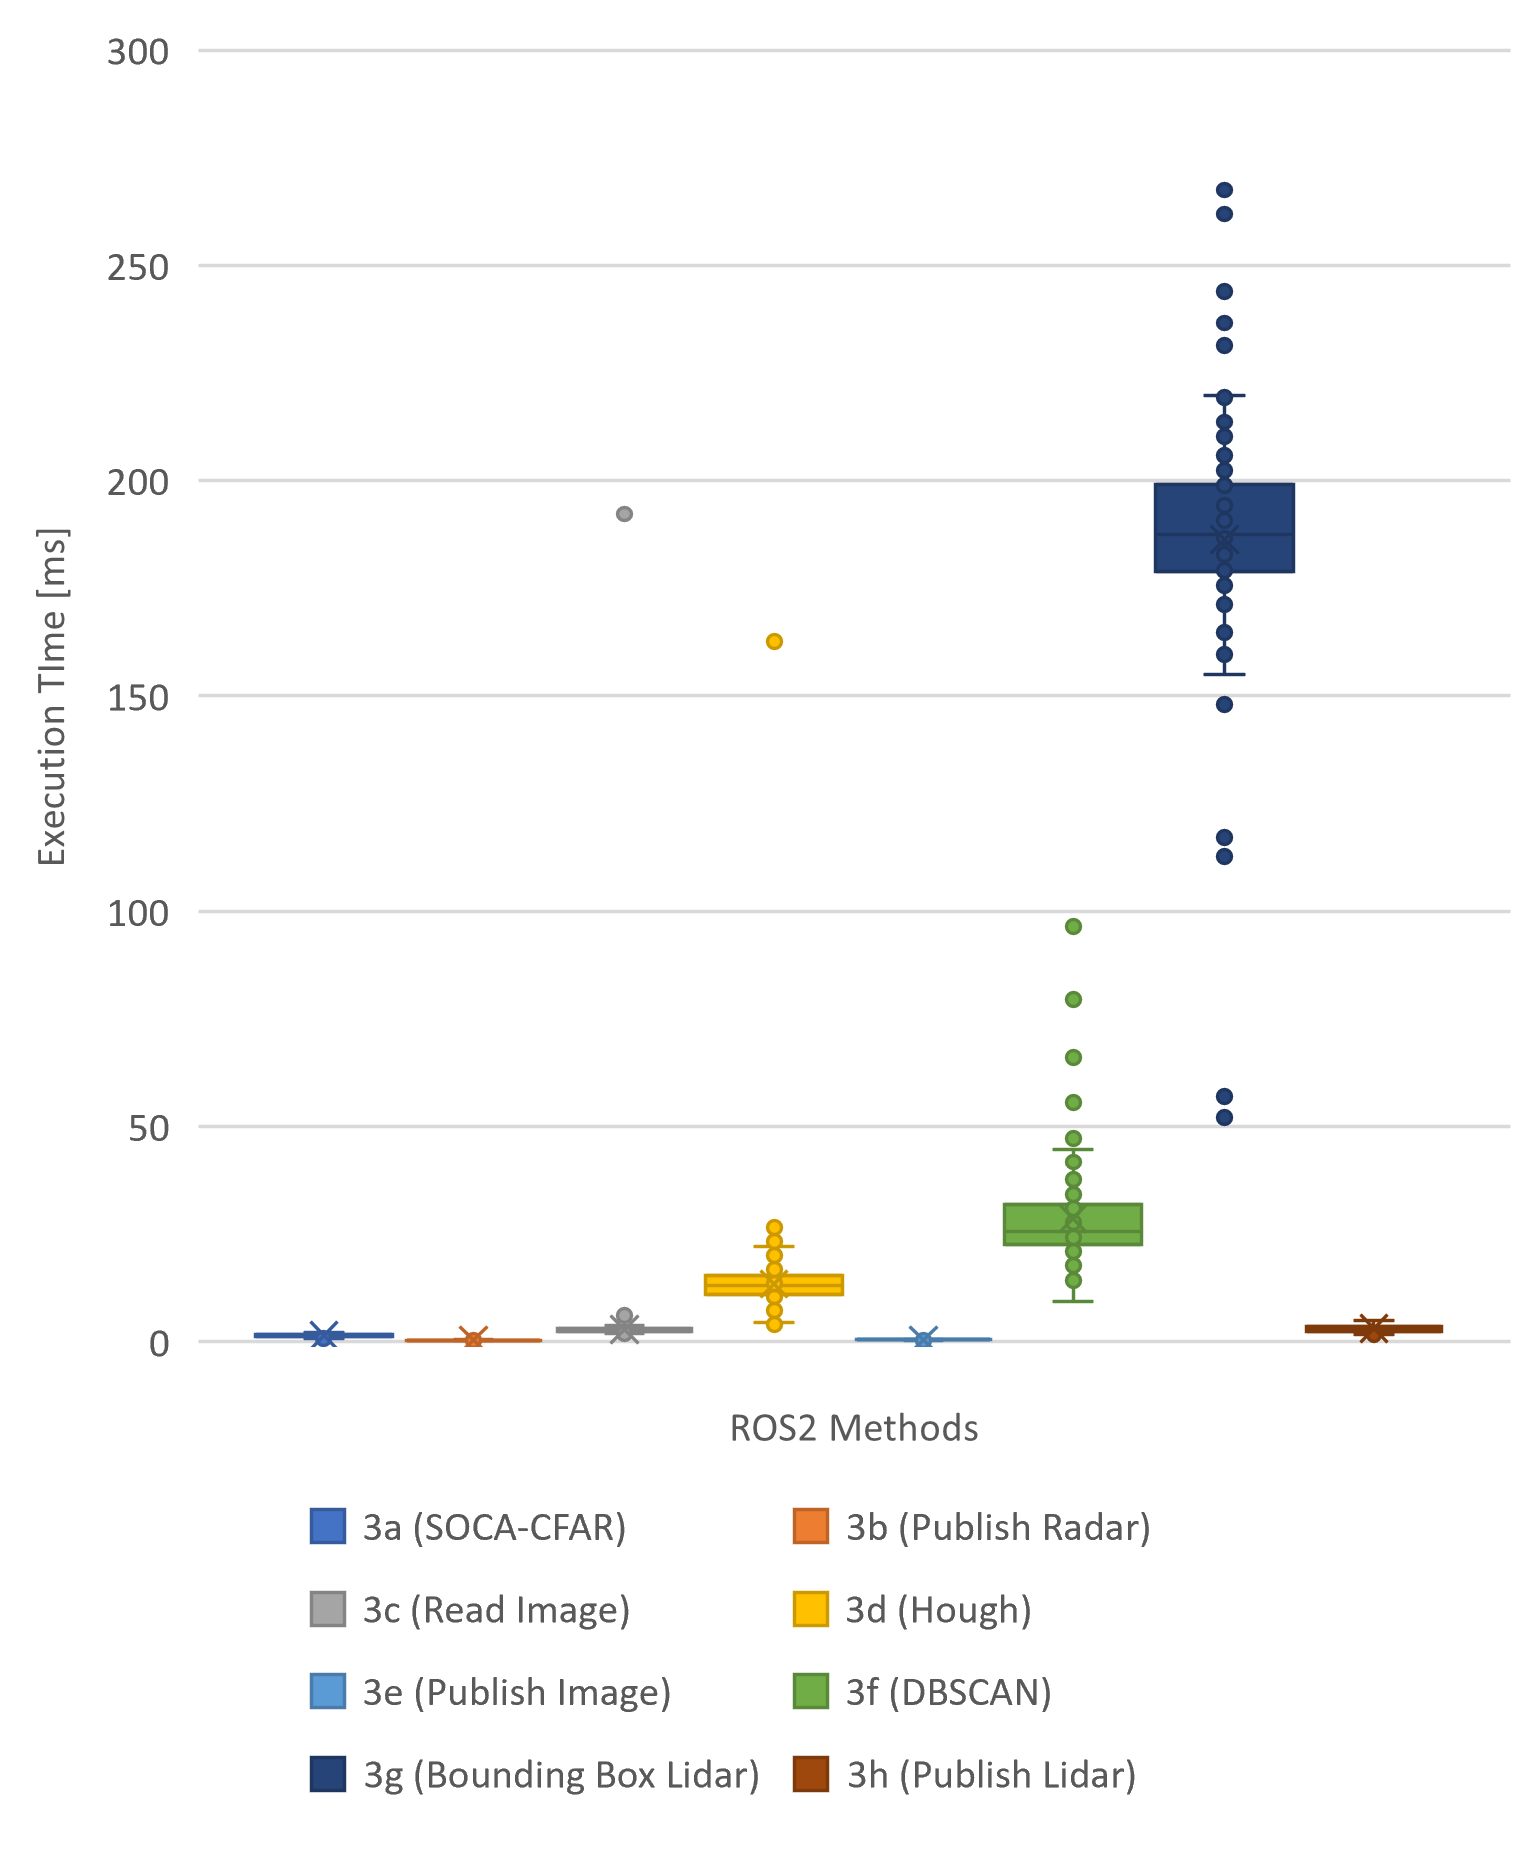
\includegraphics[height=3cm]{Bilder/ROS22.png}%
				\enskip
				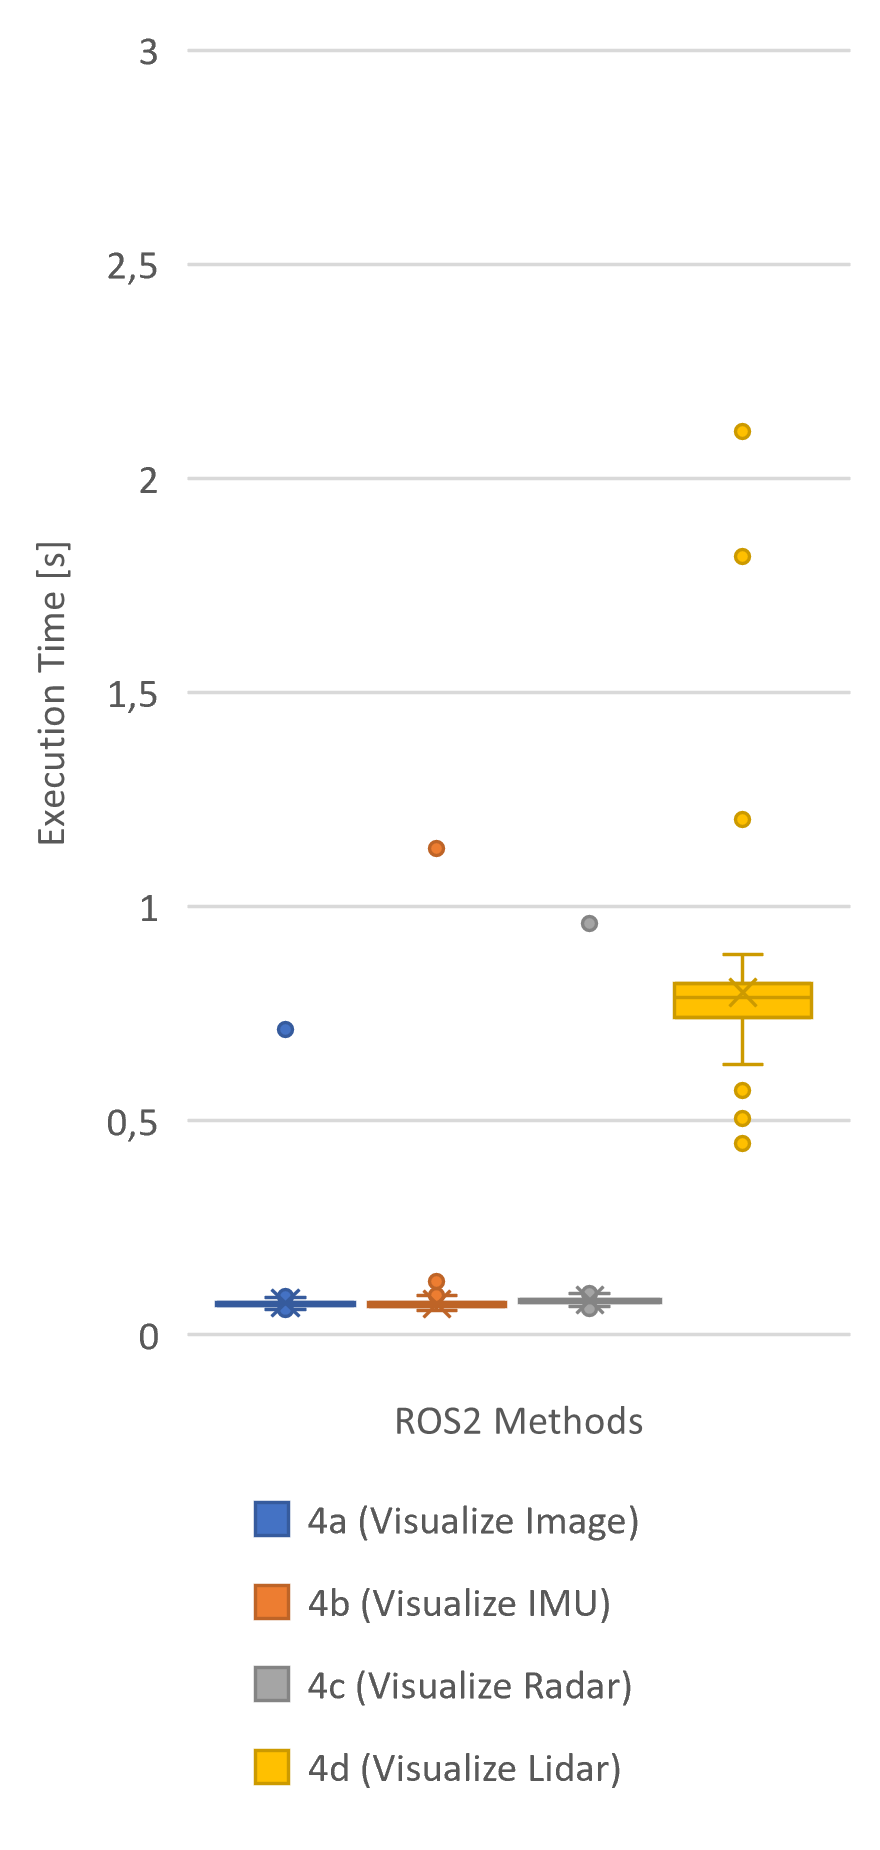
\includegraphics[height=3cm]{Bilder/ROS21.png}%
			}
			\caption{ROS2 methods time in (total of 27300 executions)}
			\label{fig_Ros21}%Label für das Referenzieren 
		\end{center}
	\end{figure}

	\section{Part Integration Test}\label{intpart}

	 Continuing with the time that is required to transmit the data, as a first step the average size of the messages that are transmitted is taken. To avoid measurements that are delayed by processing data in \ac{ROS2}, empty nodes with the only purpose of accepting data are written. In table \ref{tab_msgsize}, (5a) to (5e) show the average size of 100 message of the \ac{RADAR}, \ac{LIDAR}, \ac{IMU} and Image sensor respectively as well as the total transmitted size per second. With 285 KB/s, (5b) stands out of (5a), (5c) and (5d) and makes up a large part of the sum of messages sizes of about 291 KB/s. Considerably larger than the message size is the average intern network load of the system that is measured with the tool \textit{nload} and calculated over 100 samples. 1.62 MB/s as shown in table \ref{tab_netload} are send over the network under load of which only 24.418 KB/s are used from the operating system. The high value can be explained with the necessity of converting and resending the data between the Unity3d environment in C\# and the ROS2 environment in C++ over the Node.js framework in Java. However, a multiplication of about five relative to the total size of the messages is considered as high and can be investigated in further studies to increase the system performance and decrease the latency.\\
	 \begin{figure}[!htb]
	 	\begin{minipage}[t]{0.48\textwidth}	
	 		\begin{table}[H]	
	 			\centering
	 			\caption{Message size in ROS2}
	 			\begin{tabular}{l l } 
	 				\toprule
	 				Name  & Size  $\varnothing100$\\ 
	 				\midrule
	 				5a (Radar) & 5.78 KB/s\\
	 				5b (Lidar) & 285.37 KB/s\\
	 				5c (\ac{IMU}) & 32 B/s \\
	 				5d (Image) & 88 B/s \\\\
	 				
	 				5e Sum         & 	291.270 KB/s\\
	 				\bottomrule
	 			\end{tabular}
	 			\label{tab_msgsize}
	 		\end{table}
	 	\end{minipage}\hfill
	 	\begin{minipage}[t]{0.48\textwidth}
	 		\begin{table}[H]
	 			\centering
	 			\caption{Network Load}
	 			\begin{tabular}{l l } 
	 				\toprule
	 				Network Load & $\varnothing300s$ \\ 
	 				\midrule
	 				Idle In/Out &24.418 KB/s \\	 
	 				Publishing In/Out & 1.62 MB/s \\
	 				\bottomrule
	 			\end{tabular}
	 			\label{tab_netload}
	 		\end{table}
	 	\end{minipage}
	 \end{figure}
	 
	 Investigating the latency, to the left of figure \ref{fig_transmission}, (i) to (l) provide the values for the average transmission time from the Unity3d system to the \ac{ROS2} system. With an average of 86ms, the \ac{LIDAR} data (h) stands out from the other values but can be considered as acceptable as the \ac{LIDAR} data includes a high amount of single point values that have to be transmitted. However, more important than the average time is the reliability with which the transmission time is in a certain interval of time. Therefore, a more detailed representation of the data is shown in figure \ref{fig_transmission} to the right with a box and whiskers plot. It becomes clear that the average transmission time of the message conceal a highly scattered latency. Especially for the \ac{IMU} (5c) with only 32 B/s of data size, transmission times of above 80ms are possible with an median of below 10ms. Similar to (5c), the difference of the median to the highest latency value measured in (5b) is about 50ms. However, no requirement on the real time behaviour is set for the system and times of below 140ms are within a range that can be considered as sufficient for an adequate response in the scope of the appliance at hand. Detailing the real time definition of the appliance may be considered in further studies. 
	 
		\begin{figure}
		\begin{center}
			\resizebox{.9\textwidth}{!}{%
				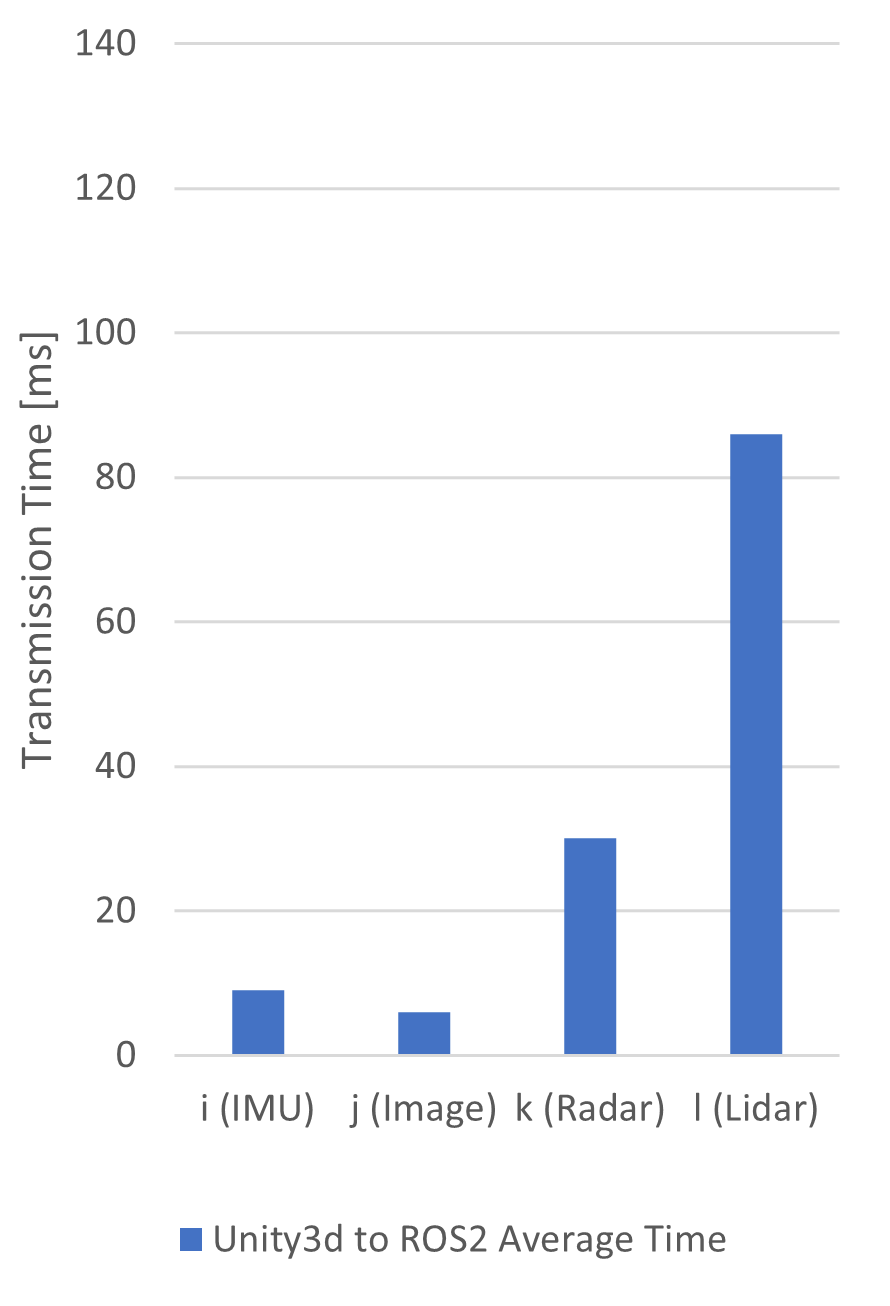
\includegraphics[height=3cm]{Bilder/TimingAver.png}%
				\enskip
				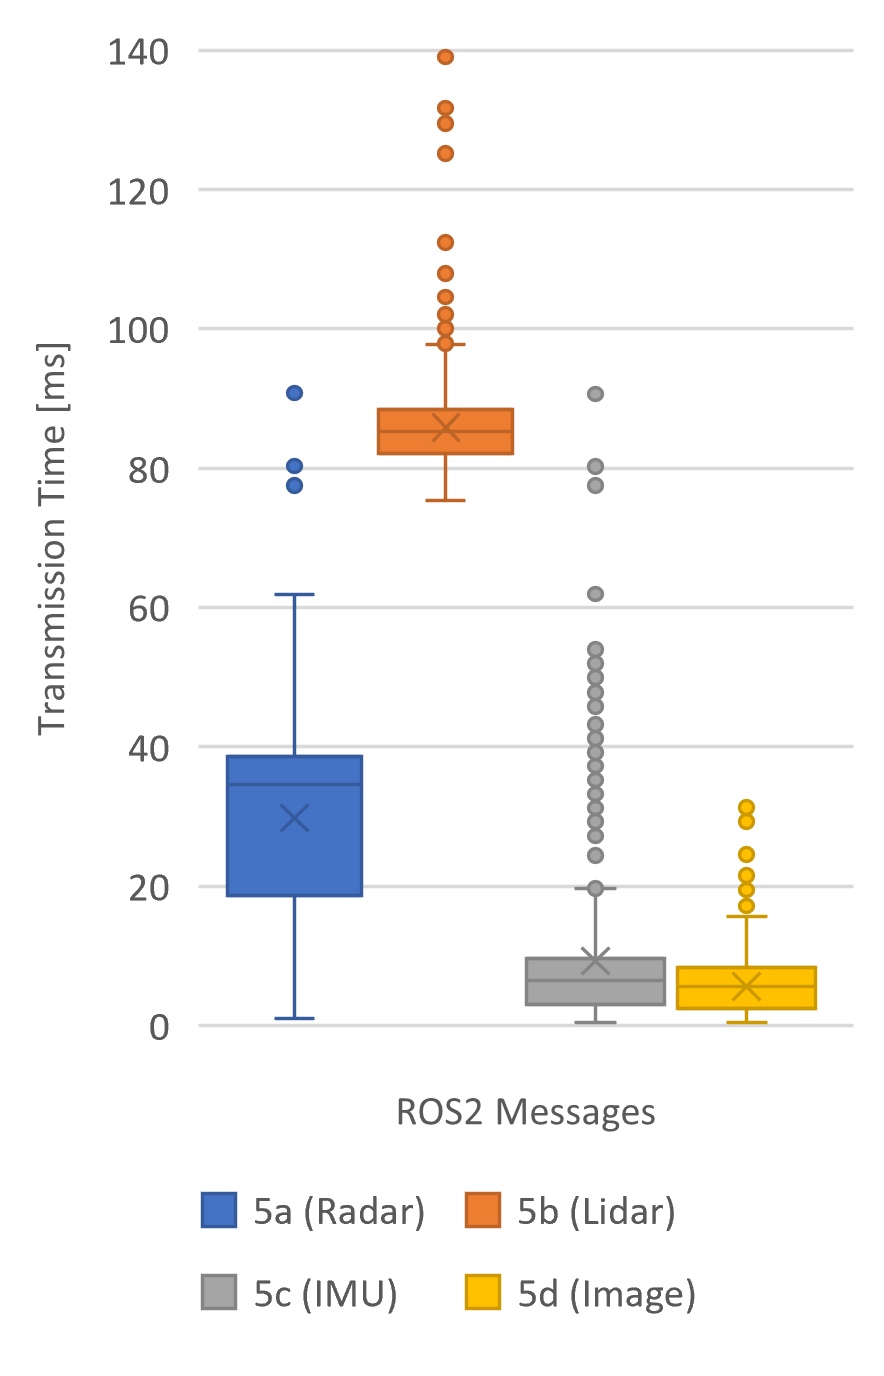
\includegraphics[height=3cm]{Bilder/Transmission.png}%
			}
			\caption{ROS2 methods time in (total of 12600 executions)}
			\label{fig_transmission}%Label für das Referenzieren 
		\end{center}
	\end{figure}
	
	\section{Validation Software} \label{validate}
	In this section, the implemented system is validated by using the proposed system architecture, the system specification and requirements defined in terms of safety. Central to the implementation is the software framework \ac{ROS2} that can be used to connect real sensors as well as virtual sensors, control actuators and share information with a control center. The library that is chosen to connect to the virtual sensors allows for a physical separation of the processing units that calculates the virtual sensors data and the subsequent processing of the data. Unity3d as the simulation environment proofed to be able to generate virtual sensor data and it is possible to resemble different types of sensors to percept the virtual environment. Therefore the chosen modules and the implemented system architecture is in compliance with the specified design. The system implementation is oriented at the V- Model and therefore complies with the demand to use a valid software safety life cycle model. Verifying the software further, the part of the regulations that relate to the design of a software framework state, that the information that result in any autonomous decision making is to be shared with the personell of the \ac{MASS} trial. The software as implemented fullfills this demand by visualizing the processed data of the sensors after each processing step.\\
	
	Continuing with a more detailed analysis, the system as implemented is tested against the criteria set in section 7.4 of \ac{VDE} 0803-3 \cite{DIN_3} and described in section \ref{Require}. A total of 14 criteria should be met in the software design and development process. In table \ref{tab_veri}, the criteria of the test that is conducted is given with the result being positive or negative. To start with the first two tests that are specified, it can be concluded that there no fault in the concept is detectable (1) and the overall system is designed with a focus on easy comprehensibility (2). With the utilization of \ac{ROS2} as a central framework, a deterministic behaviour of the data processing can be ensured (3). As only the Unity3d environment is used in the system and therefore influences of a real environment are missing, criteria (4) can not be evaluated. Both Unity3d and \ac{ROS2} provide possibilities to ad or replace components where required through the asset store in the first case and packages in the latter. This option results in a modular (5) and changeable code (6). By making use of classes and methods, the code in Unity3d is divided into several submodules that are easily testable. However, the methods of one class are dependent on each other. Therefore testing each method for itself requires a considerable amount of additional code that simulate the respective methods before the method that is to be tested. The same is the case for the code in \ac{ROS2}. With a division into nodes, classes and methods, methods are still dependent on each other. However, as the separate testing is not a requirement, criteria (7) and (8) are considered to be met. By making use of a structured process oriented at the V-model throughout every aspect of the system design is  documented which includes the intended design of the system (9), the integration test (10) that falls together with the module test (11) and the safety validation. In the module implementation, a summary is provided by every class and method that is written to ease the understanding of the purpose of the code (13). The author of the code is documented, too (14). It is noted that no liability or responsibility is taken for the code.\\
	
	

		\begin{table}[H]
		\centering	
		\caption{Safety criteria in system validation}
		\begin{tabular}{ l l } 
	\toprule
	Criteria & Criteria met \\
	\midrule
	(1)  Without faults in the concept  &  \cmark \\
	(2)  Easily comprehensible 			&   \cmark\\
	(3)  Display a deterministic behaviour &\cmark\\
	(4)  Fault tolerant in the event of external events &\xmark$^1$\\
	(5)  Modularity 					&\cmark\\
	(6)  Changeable code 				&\cmark\\
	(7)  Divided into several more detailed submodules &\cmark $^2$\\
	(8)	 Testable 						&\cmark\\
	(9)  Intended design of the system documented &\cmark\\
	(10) Integration Test documented	&\cmark\\
	(11) Module test documented 		&\cmark\\
	(12) Safety validation of the system is documented &\cmark\\
	(13) Software is documented &\cmark\\
	(14) Responsibility is documented  &\cmark $^3$\\
	\bottomrule
	
	\multicolumn{2}{l}{\small $^1$ no test specified, only the simulation is used as a test environment } \\
	\multicolumn{2}{l}{\small $^2$ submodules are dependent on each other, separate testing requires more effort } \\
	\multicolumn{2}{l}{\small $^3$ translates to the documentation of the author of the code} \\
\end{tabular}
\label{tab_veri}
\end{table}

